\section{Test af styresystem}
Styresystemets enkelte moduler testes hver for sig for at verificere at de fungerer efter hensigten. Følgende afsnit vil derfor gennemgå accepttesten for styresystemet modul for modul.    
%
\subsection{Test af stereovolumenkontrol}
For at verificere, at stereovolumenkontrollen justerer lydtryksniveauet efter hensigten er det nødvendigt at undersøge, om justeringen af volumen faktisk resulterer i en lineær udvikling. Dette blev dog allerede belyst i \fullref{Volumenkontrol}, hvor hensigten var at kompensere for et fladt forløb ved lave og høje frekvenser, inden den endelige stereovolumenkontrol skulle bygges. Løsningen på dette problem var at placere modstande på hver side af potentiometeret, hvilket gav en mere favorabel udvikling ved justering af potentiometeret.\\

\noindent
I det færdige system er det vigtigt, at alle frekvenser afspilles lige højt, uanset spændingen over potentiometeret. Frekvensresponsen for udvalgte spændinger måles derfor, for at undersøge, om dette er tilfældet, hvilket er illustreret på \autoref{fig:VolumenkontrolTest}. Ønsket er at opnå en flad linje i forsøgsdata, da det netop vil indikere, at alle frekvenser afspilles lige højt. Som det fremgår af forsøgsdata, synes dette til gengæld ikke at være tilfældet for alle spændinger. Når volumenkontrollen er drejet til endepunkterne, og der er en meget lav eller meget høj spænding over potentiometeret, er der ikke noget, der tilnærmelsesvist kan kaldes en flad linje igennem frekvensspektrummet. Dette har dog ikke den største betydning, da der netop er tale om volumenkontrollens yderpunkter. Mere interessant er det at fokusere på, hvordan den opfører sig inden for potentiometerets mere centrale område, da det er vigtigt, hvordan den opfører sig ved de lydtryksniveauer, hvor der faktisk lyttes til musik. Her synes der at være klart pænere testresultater, der nærmer sig regulære flade linjer. Dog afviger disse stadig med $0.5dB$, hvor det højfrekvente område bliver forstærket lidt, og det lavfrekvente område bliver dæmpet. Dette synes dog ikke at være af stor nok betydning, og volumenkontrollen vurderes derfor stadig til at være udmærket at anvende.
%
\newpage
\noindent
%
\begin{figure}[H]
	\centering
	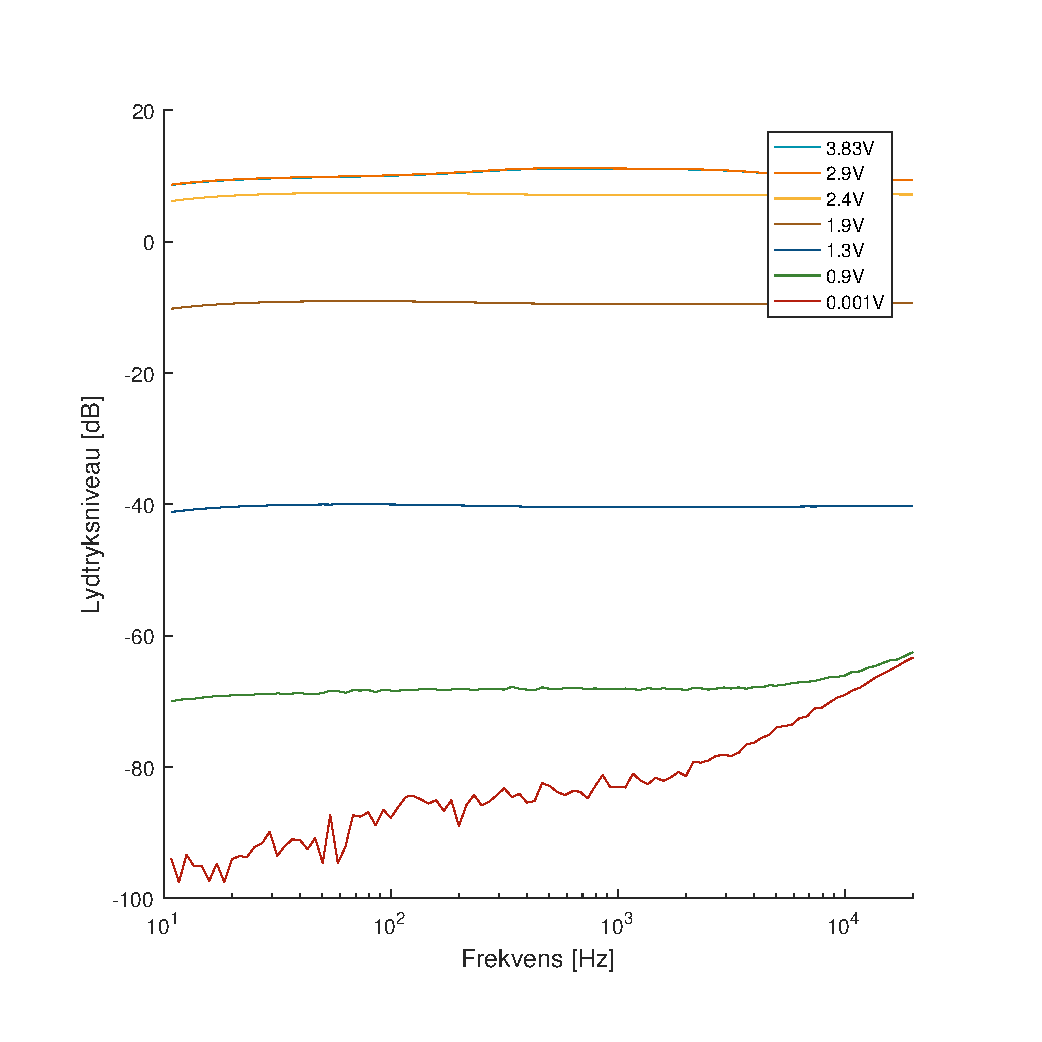
\includegraphics[resolution=300,width=\textwidth]{Figure/VolumeControl.pdf}
	\caption{Frekvensanalyse af volumenkontrollen.}
	\label{fig:VolumenkontrolTest}
\end{figure}
\noindent
%
I sammenhæng med en undersøgelse af frekvensresponsen, fokuseres der også på, hvor rent outputsignalet er. Hvis signalet er meget forvrænget, kan det indikere, at volumenkontrollen ikke fungerer efter hensigten, og det vil i såfald være nødvendigt at foretage modificeringer. Der undersøges således THD ved forskellige spændinger, hvor det fremgår fra kredsløbets datablad, at dette gerne skal ligge på $0.3\%$, \parencite[][2]{PDF:VolumeControl}.
%
\begin{table}[H]
\centering
\begin{tabular}{|l|l|l|l|l|l|l|l|}
\hline
V & 0.001 & 0.90 & 1.30 & 1.90 & 2.40 & 2.90 & 3.83 \\ \hline
THD \% & 28.26 & 3.66 & 0.26 & 0.15 & 0.81 & 31.94 & 38.47 \\ \hline
\end{tabular}
\caption{Den målte THD ved udvalgte spændinger over potentiometeret.}
\label{tab:VolumenkontrolTHD}
\end{table}
%
Resultatet af målingerne er illustreret i \autoref{tab:VolumenkontrolTHD}, hvor det fremgår, at de lave og høje spændinger over potentiometeret har en alt for høj THD. Dette styrker dog bare yderligere, fordelen ved at placere modstande i hver ende af potentiometeret, så det vil bevæge sig fra en spænding i den ene ende på $0.9$V til en spænding på $2.9$V i den anden. Ved spændingerne imellem opfører volumenkontrollen sig stort set efter hensigten, men der fremgår dog en afvigelse ved målingen for $2.40$V, jævnfør \autoref{tab:VolumenkontrolTHD}. Det betyder, at yderligt fokus på volumenkontrollen kunne have været fornuftigt, men denne afvigelse vurderes samtidig ikke som værende alarmerende, så volumenkontrollen synes stadig at være anvendelig.
%
\subsection{Test af A/D-konverter}
Hensigten med A/D-konverteren er, at den ud fra en analog spænding på indgangsterminalen skal levere et digitalt binært outputsignal, der svarer til den pågældende indgangsspænding, hvilket fremgår af §2.3 i \fullref{OpsummeringAfSpecifikkeSystemkrav}. For at verificere dette, testes A/D konverteren ved at måle på kredsløbets outputterminaler, DB7, DB6, DB5 og DB4, samtidig med at spændingen på inputterminalen, $V_{in(+)}$, gradvist justeres. Data fra testen fremgår af \fullref{tab:ADkonverter}. Som det fremgår af \fullref{tab:ADkonverter}, kan det bekræftes, at A/D-Konverteren kan modtage en analog spænding på indgangen og konvertere dette til en digital binær talkode. De forskellige outputs er enten givet ved et 1-tal, der svarer til et højt output, eller et 0-tal, der svarer til et lavt output.          
%
\begin{table}[H]
\centering
\begin{tabular}{|c|c|c|c|c|}
\hline
\multicolumn{5}{|c|}{A/D konverter}  \\ \hline
Input  & \multicolumn{4}{c|}{Output} \\ \hline
Vin(+) & MSB - DB7 & DB6 & DB5 & DB4 \\ \hline
0      & 0         & 0   & 0   & 0   \\ \hline
0,34   & 0         & 0   & 0   & 1   \\ \hline
0,65   & 0         & 0   & 1   & 0   \\ \hline
0,97   & 0         & 0   & 1   & 1   \\ \hline
1,27   & 0         & 1   & 0   & 0   \\ \hline
1,59   & 0         & 1   & 0   & 1   \\ \hline
1,91   & 0         & 1   & 1   & 0   \\ \hline
2,22   & 0         & 1   & 1   & 1   \\ \hline
2,54   & 1         & 0   & 0   & 0   \\ \hline
2,84   & 1         & 0   & 0   & 1   \\ \hline
3,16   & 1         & 0   & 1   & 0   \\ \hline
3,48   & 1         & 0   & 1   & 1   \\ \hline
3,79   & 1         & 1   & 0   & 0   \\ \hline
4,11   & 1         & 1   & 0   & 1   \\ \hline
\end{tabular}
\caption{Data fra accepttesten af A/D konverteren.}
\label{tab:ADkonverter}
\end{table}
%
\subsection{Test af komparator}
Hensigten med komparatoren er, at den skal levere et digitalt højt output, hvis spændingen på indgangsterminalen er over referencen og et digitalt lavt output, hvis spændingen er under referencen, hvilket også fremgår af §2.4 i \fullref{OpsummeringAfSpecifikkeSystemkrav}. Dette verificeres med en accepttest, hvor der måles på komparatorens udgangsterminal, imens spændingen på indgangsterminalen gradvist justeres. Resultatet af dette fremgår af \fullref{tab:Komparator}, hvor det netop er tydeligt, at komparatoren leverer et højt digitalt output, når spændingen på indgangsterminalen er over referencen. Samtidig leverer komparatoren et lavt digitalt output, når spændingen på indgangsterminalen er under referencen.
%
\begin{table}[H]
\centering
\begin{tabular}{|c|c|}
\hline
\multicolumn{2}{|c|}{Komparator} \\ \hline
Input           & Output         \\ \hline
2,09            & 5              \\ \hline
1               & 4,98           \\ \hline
0,09            & 4,96           \\ \hline
-0,016          & 0,046          \\ \hline
-1              & 0,046          \\ \hline
-1,969          & 0,046          \\ \hline
\end{tabular}
\caption{Accepttest af komparator.}
\label{tab:Komparator}
\end{table}
%
\subsection{Test af dobbeltensretter}
Hensigten med dobbeltensretteren er, at den skal kunne modtage en positiv eller negativ spænding på indgangsterminalen, og herefter skal den så kunne levere den numeriske værdi af amplitudens spænding på udgangsterminalen. Dette fremgår af §2.5 i \fullref{OpsummeringAfSpecifikkeSystemkrav}. Testning af dette foregår ved, at måle på dobbeltensretterens udgangsterminal, imens spændingen på indgangsterminalen gradvist justeres fra at være positiv til at være negativ. Resultatet af målingerne fremgår af \autoref{tab:Dobbeltensretter}, hvor alle spændingerne på indgangsterminalen giver et positivt output, uanset om inputtet er positivt eller negativt.
%
\begin{table}[H]
\centering
\begin{tabular}{|c|c|}
\hline
\multicolumn{2}{|c|}{Dobbeltensretter} \\ \hline
Input              & Output            \\ \hline
2,031              & 4,31              \\ \hline
0,913              & 1,933             \\ \hline
0,897              & 1,899             \\ \hline
0,8                & 1,693             \\ \hline
0,7                & 1,478             \\ \hline
0,6                & 1,266             \\ \hline
0,5                & 1,053             \\ \hline
0,401              & 0,841             \\ \hline
0,399              & 0,623             \\ \hline
0,2                & 0,412             \\ \hline
0,1                & 0,203             \\ \hline
-0,102             & 0,231             \\ \hline
-0,204             & 0,457             \\ \hline
-0,3               & 0,671             \\ \hline
-0,398             & 0,888             \\ \hline
-0,504             & 1,122             \\ \hline
-0,604             & 1,342             \\ \hline
-0,702             & 1,56              \\ \hline
-0,806             & 1,791             \\ \hline
-0,899             & 1,997             \\ \hline
-1,005             & 2,232             \\ \hline
-1,1               & 2,439             \\ \hline
-2,012             & 4,33              \\ \hline
\end{tabular}
\caption{Accepttest af dobbeltensretteren.}
\label{tab:Dobbeltensretter}
\end{table}
%
\subsection{Test af differensforstærker}
Hensigten med differensforstærkeren er, at den skal modtage en spænding på hver af de to indgangsterminaler og herefter levere differencen mellem disse spændinger på udgangsterminalen, hvilket også fremgår af §2.6 i \fullref{OpsummeringAfSpecifikkeSystemkrav}. Testning af dette er udført ved at måle på differensforstærkerens udgangsterminal, imens spændinger på indgangsterminalerne gradvist justeres i forhold til hinanden. Resultatet af testen fremgår i \autoref{tab:Differensforstaerker}, hvor det er tydeligt, at outputtet leverer differencen mellem de to inputs.
%
\begin{table}[H]
\centering
\begin{tabular}{|c|c|c|}
\hline
\multicolumn{3}{|c|}{Differensforstærker}              \\ \hline
Volumenpotentiometer & Referencepotentiometer & Output \\ \hline
0,872                  & 2,887                & -2,012 \\ \hline
0,872                   & 1,895               & -1,023 \\ \hline
0,874                   & 0,874               & 0      \\ \hline
1,874                   & 0,872               & 1,004  \\ \hline
2,907                   & 0,873               & 2,033  \\ \hline
\end{tabular}
\caption{Accepttest af differensforstærkeren.}
\label{tab:Differensforstaerker}
\end{table}
%
\subsection{Test af multiplekser}
Multipleksernes kontaktfunktioner, som enten leder lydsignalet igennem eller udenom filtrene styres som tidligere nævnt i \fullref{OpsummeringAfSpecifikkeSystemkrav} ved hjælp af et digitalt binært signal fra A/D konverteren. For at vide nøjagtigt hvorvidt kontaktfunktionerne faktisk opfører sig efter hensigten, er det nødvendigt at teste modulet via en acceptest. Verificeringen af modulet isoleret har dog vist sig at være kompliceret. Modulet er derfor blevet testet indirekte, hvilket betyder at en direkte måling på multipleksernes kontaktfunktioner ikke er foretaget. I stedet måles resultatet af at kontaktfunktionerne faktisk har opført sig efter hensigten ved hjælp af A/D konverteren og det behandlede lydsignal. \autoref{tab:multiplekser} og \autoref{tab:multiplekserIgen} gengiver resultatet fra testen.\\        
%
\begin{table}[H]
\centering
\begin{tabular}{|l|l|l|l|l|l|l|l|}
\hline
& Input & Output & Bits &  &  &  &  \\ \hline
Frekvens & Spænding & Spænding & Komparator & MSB-DB7 & DB6 & DB5 & DB4 \\ \hline
20Hz & 100mV & 13mV & 0 & 0 & 0 & 0 & 0 \\ \hline
20Hz & 100mV & 17mV & 0 & 0 & 0 & 0 & 1 \\ \hline
20Hz & 100mV & 26mV & 0 & 0 & 0 & 1 & 0 \\ \hline
20Hz & 100mV & 36.8mV & 0 & 0 & 0 & 1 & 1 \\ \hline
20Hz & 100mV & 47.6mV & 0 & 0 & 1 & 0 & 0 \\ \hline
20Hz & 100mV & 66mV & 0 & 0 & 1 & 0 & 1 \\ \hline
20Hz & 100mV & 88mV & 0 & 0 & 1 & 1 & 0 \\ \hline
20Hz & 100mV & 118mV & 0 & 0 & 1 & 1 & 1 \\ \hline
20Hz & 100mV & 134mV & 0 & 1 & 0 & 0 & 0 \\ \hline
\end{tabular}
\caption{Resultat af forstærkning på udgangsspændings i forhold til indgangsspænding, ved 20Hz, fra indirekte accepttest af multiplekserne.}
\label{tab:multiplekser}
\end{table}
%
\begin{table}[H]
\centering
\begin{tabular}{|l|l|l|l|l|l|l|l|}
\hline
& Input & Output & Bits &  &  &  &  \\ \hline
Frekvens & Spænding & Spænding & Komparator & MSB-DB7 & DB6 & DB5 & DB4 \\ \hline
20Hz & 736mV & 100mV & 0 & 0 & 0 & 0 & 0 \\ \hline
20Hz & 736mV & 132mV & 0 & 0 & 0 & 0 & 1 \\ \hline
20Hz & 736mV & 196mV & 0 & 0 & 0 & 1 & 0 \\ \hline
20Hz & 736mV & 260mV & 0 & 0 & 0 & 1 & 1 \\ \hline
20Hz & 736mV & 352mV & 0 & 0 & 1 & 0 & 0 \\ \hline
20Hz & 736mV & 472mV & 0 & 0 & 1 & 0 & 1 \\ \hline
20Hz & 736mV & 640mV & 0 & 0 & 1 & 1 & 0 \\ \hline
20Hz & 736mV & 860mV & 0 & 0 & 1 & 1 & 1 \\ \hline
20Hz & 736mV & 1000mV & 0 & 1 & 0 & 0 & 0 \\ \hline
\end{tabular}
\caption{Resultat af forstærkningen på udgangsspænding i forhold til indgangsspænding, ved 20Hz, fra indirekte accepttest af multiplekserne.}
\label{tab:multiplekserIgen}
\end{table}
\noindent
Testen er fortaget ved en fast frekvens på 20Hz. Volumenpotentiometeret er ligeledes fikseret omkring den samme spænding. Det eneste der ændres er derfor referencepotentiometeret. Til at starte med er referencepotentiometeret i sin yderste position, svarende til den laveste reference, hvorfor inputsignalet dæmpes. I takt med at der skrues op for referencepotentiometeret ændres forstærkningen. Forstærkningen ændres som forventet i forhold til A/D konverterens digitale output. Det antages derfor at multipleksernes kontaktfunktion virker efter hensigten, selvom accepttesten ikke direkte kan verificere dette.
